\documentclass[dvipdfmx,11pt]{beamer}
\usepackage{lipsum}
\usetheme{verona}
\usepackage{bxdpx-beamer}
\usepackage{pxjahyper}
\usepackage{minijs}
\usepackage{mathpazo}
\usepackage{amsmath,amssymb}
\usepackage{graphicx}
\usepackage{array}
\usepackage{tikz}
\usepackage{wrapfig}
\usepackage{float}
\usepackage{here}
\usepackage{lscape}
\usepackage{ascmac}
\renewcommand{\kanjifamilydefault}{\gtdefault}
\hypersetup{% hyperrefオプションリスト
 setpagesize=false,
 bookmarksnumbered=true,%
 bookmarksopen=true,%
 colorlinks=true,%
 linkcolor=blue,
 citecolor=blue,
 urlcolor = magenta
}
\setbeamertemplate{navigation symbols}{}

\title[Ang (2021, QJE)]{The Effects of Police Violence on Inner-City Students}
\subtitle{Ang (2021, Quartery Journal of Economics)}
\author[Reviewed by R.TANJI]{Reviewed by Reio TANJI}
\date{Jan 13th, 2022 \\ Ohtake-Sasaki Seminar}
\institute[]{Osaka University, Graduate School of Economics}

\begin{document}
\begin{frame}\frametitle{}
\titlepage
\end{frame}

\begin{frame}{Abstract}
  \begin{itemize}
    \item The paper documents racially disparate effects of \textbf{officer-involved killings} occur on the educational and psychological well-being of Los Angeles public high school students.
    \begin{itemize}
      \item In the United States, there occurs nearly 1,000 officer-involved killings.
    \end{itemize}
    \item Exploits hyperlocal variation in how close students live to a killing.
    \item Results: Exposure to police violence leads to
    \begin{itemize}
      \item persistent decreases in GPA
      \item increased in cidence of emotional disturbance
      \item lower rates of high school completion and college enrollment.
    \end{itemize}
    \item These effects are driven entirely by black and Hispanic students in response to
    \begin{itemize}
      \item police killings of other minorities
      \item incidents involving unarmed individuals
    \end{itemize}
  \end{itemize}
\end{frame}

\begin{frame}{}
  \begin{figure}
    \centering
    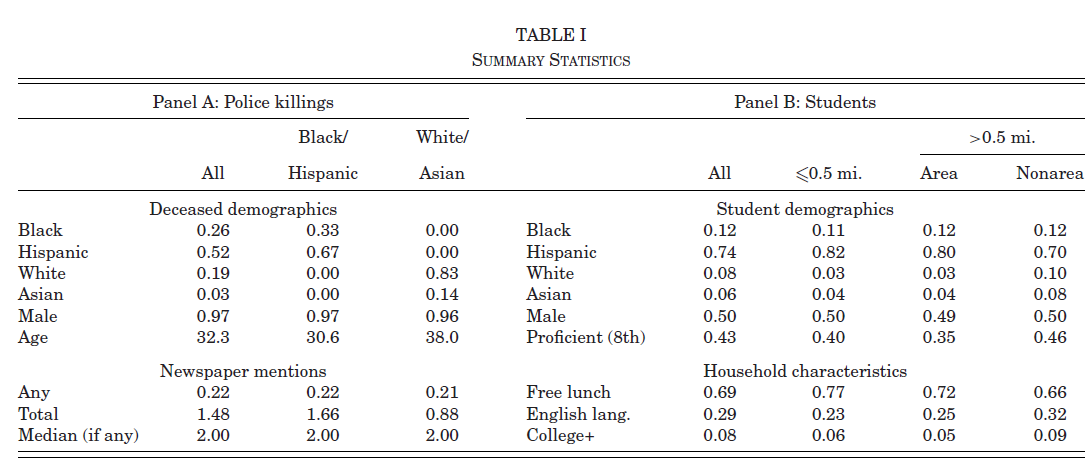
\includegraphics[scale = .6]{fig_tab/os20220113/T1}
  \end{figure}
\end{frame}

\end{document}
